In this chapter we will show the simulations conducted to evaluate the “Consensus
Algotithm”.

As said in the capter \ref{chap:system_architecture}, the software used is Gazebo.
We run SITL (Software in the loop) simulations, through the utilities provided by
the PX4 firmware. Indeed, it provides models of the main topologies of aerial vehicles,
such as plane, VTOL, Tailsitter VTOL and quadrotor.
We will use the quadrotor model called Iris, which can be shown in the picture \ref{fig:iris_model}.

\begin{figure}
\centering
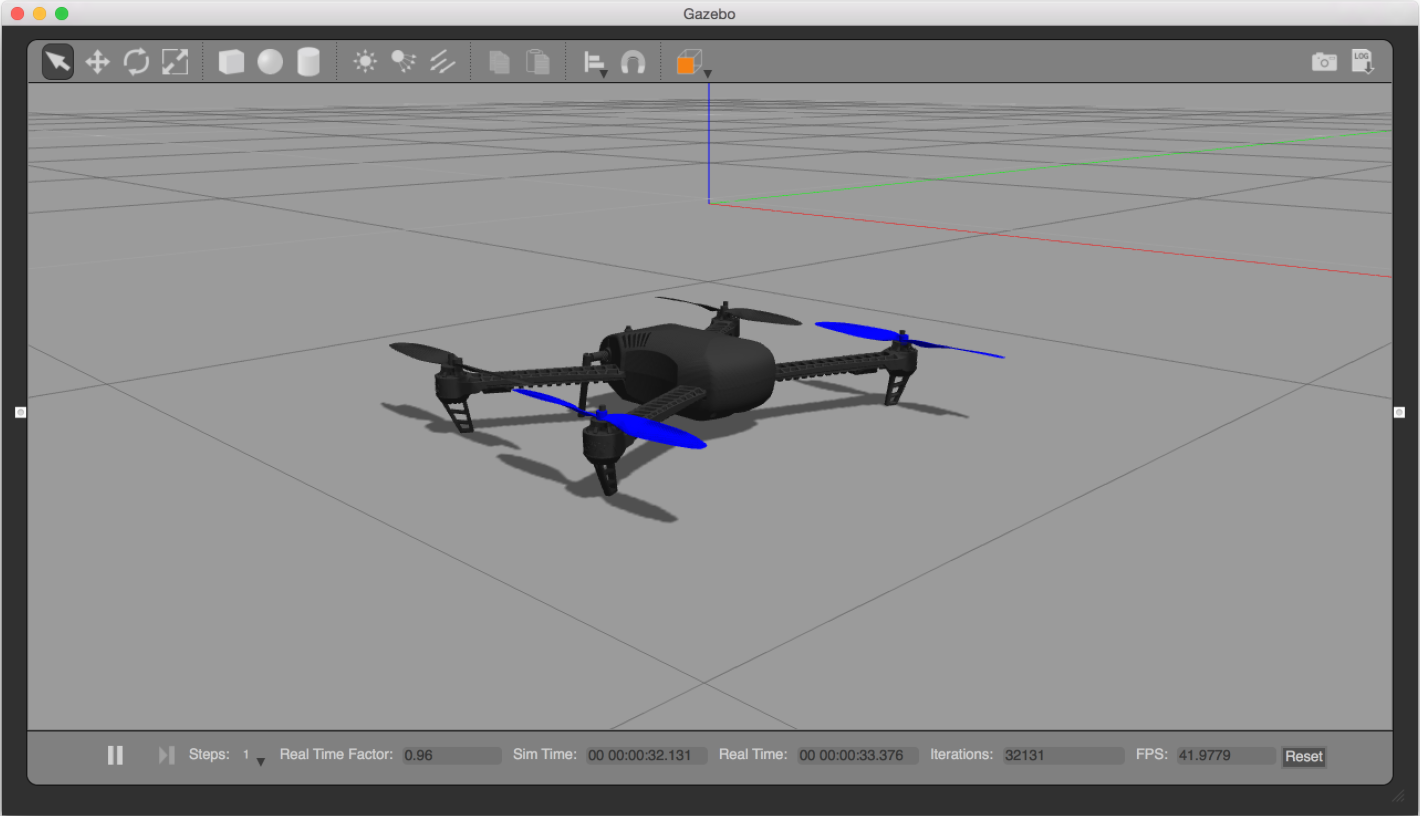
\includegraphics[width=0.9\textwidth]{chapters/chapter-04/figures/iris_model.png}
\caption{Iris model}
\label{fig:iris_model}
\end{figure}

The PX4 firmware is run on a simulated hardware and all the ROS nodes are executed
on the same computer. The physics is simulated by Gazebo and all the components
are interfaced through Gazebo plugins. In this way, the model can interact with
all the external simulated components.

The Gazebo model is specified, using SDF language, in a Gazebo model file.
All the dynamic parameters are listed in this file and also the geometry part
is stated.

The simulations that we will show are of three kinds. First, we present only
the trajectory following problem of a formation of two drones.
In the second simulation, we send a disturbance to one of the drones and we stop it
in its position. Third, we introduce a disturbance which makes one of the drones to
go back following in the reverse order its trajectory.
We see how the “Consensus algorithm” reacts to these disturbances and forces the other
drone to preserve the formation.
We use only two drones because of the computational load of the simulation, but the
concept can be extended freely to an arbitrary number of drones.

\section{Trajectory following}

The simulation is composed by two drones and the trajectory of the mission is shown
in \ref{fig:trajectory}.

\begin{figure}
\centering
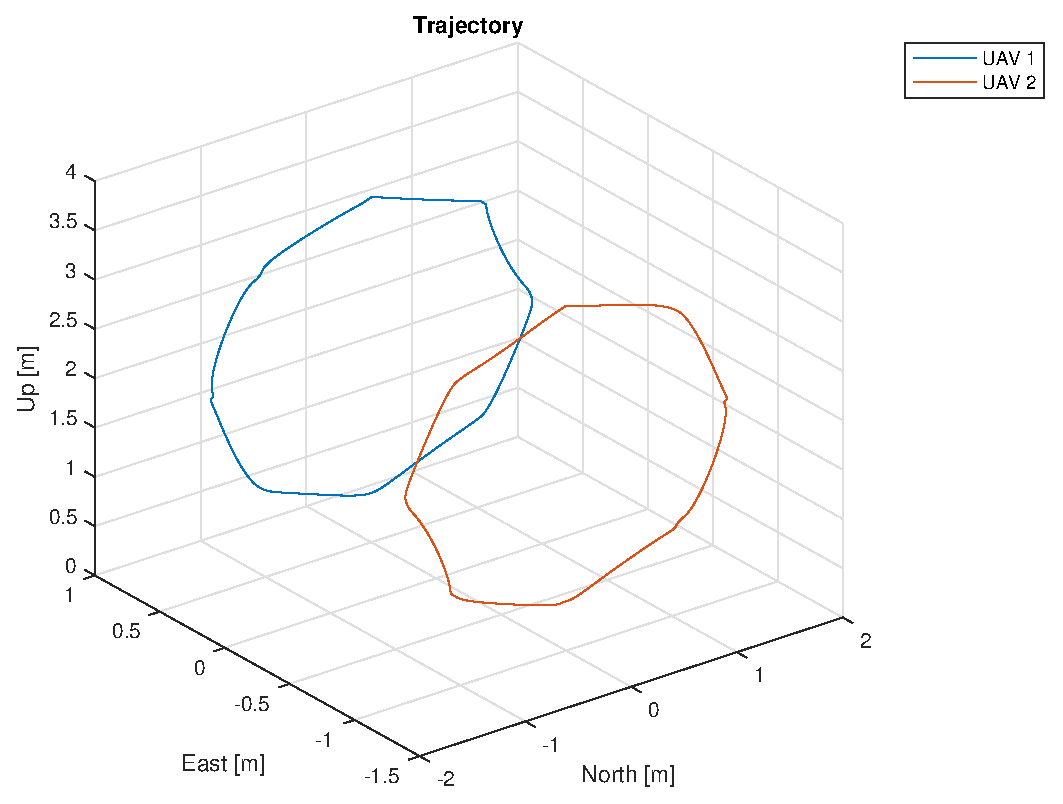
\includegraphics[width=0.7\textwidth]{chapters/chapter-04/figures/trajectory.eps}
\caption{Trajectory}
\label{fig:trajectory}
\end{figure}

Both the drones start in the upper point of their circle and then they move along the
trajectory in opposite directions. The mission terminates when both the drones reach
their starting point.
The evolution of the trajectory during time of the first drone can be seen in the figure
\ref{fig:trajectory_during_time}.

\begin{figure}
\centering
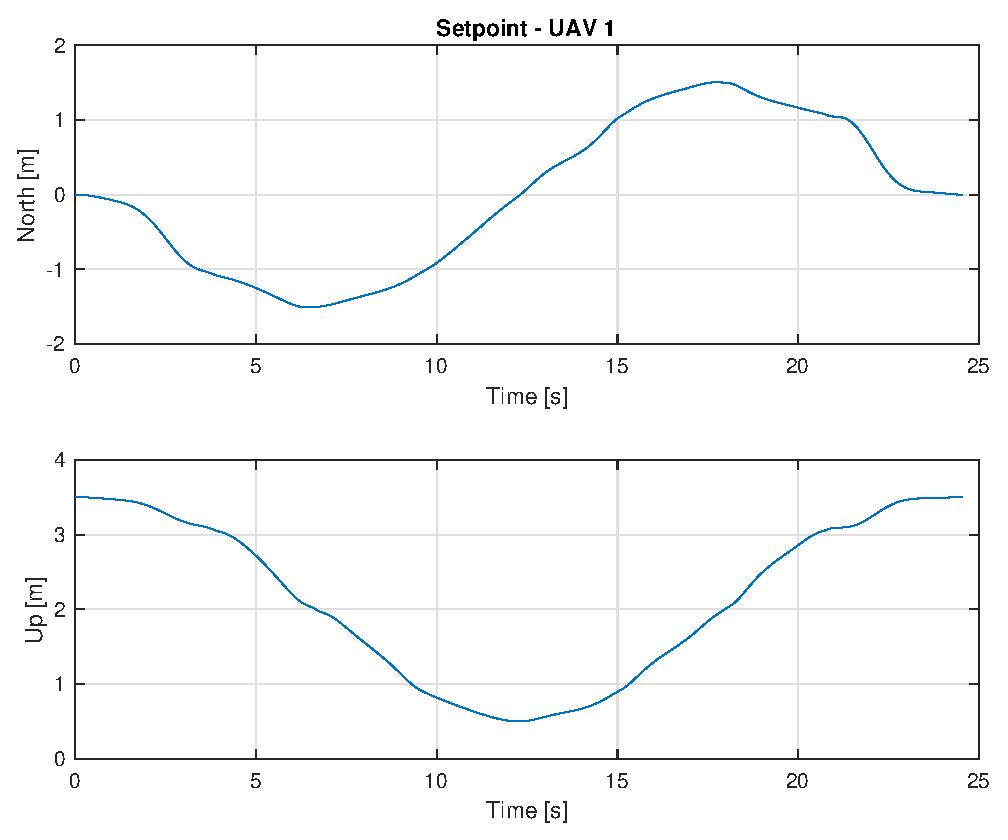
\includegraphics[width=0.7\textwidth]{chapters/chapter-04/figures/pos.eps}
\caption{Evolution of the trajectory during time of the first drone}
\label{fig:trajectory_during_time}
\end{figure}

Now we can see how the two drones follow their trajectory. It is shown in the figures
\ref{fig:following_1} and \ref{fig:following_2}.

\begin{figure}
\centering
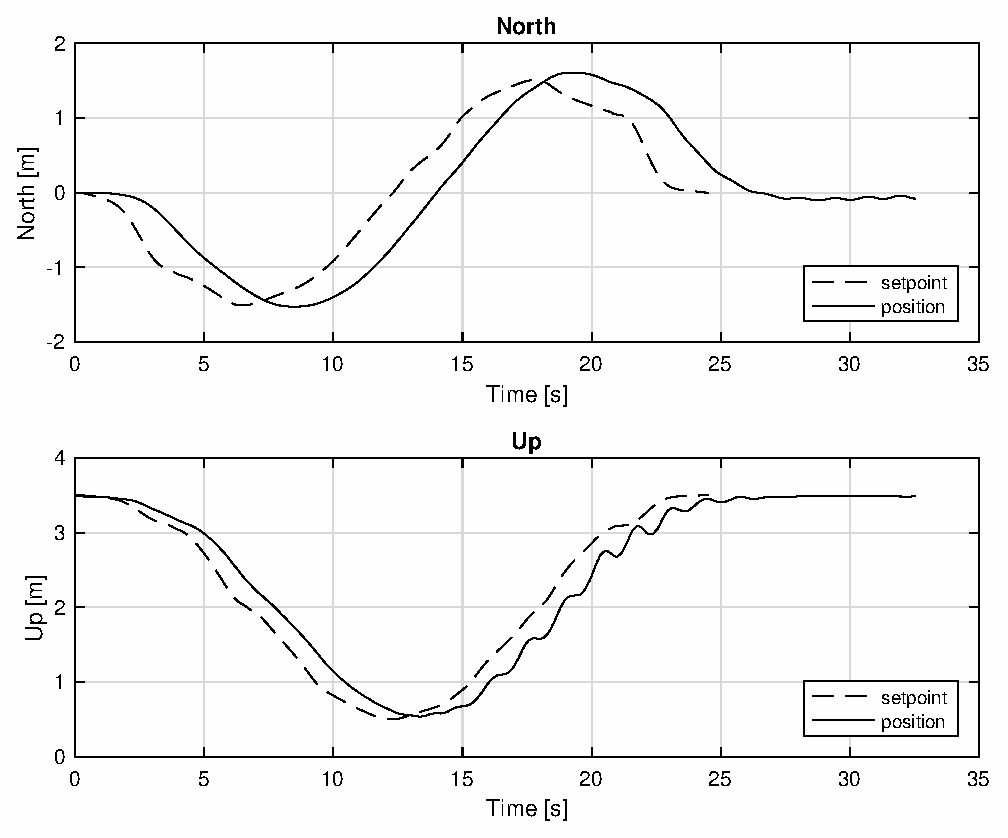
\includegraphics[width=0.7\linewidth]{chapters/chapter-04/figures/following_1.eps}
\caption{Target following drone 1}
\label{fig:following_1}
\end{figure}

\begin{figure}
\centering
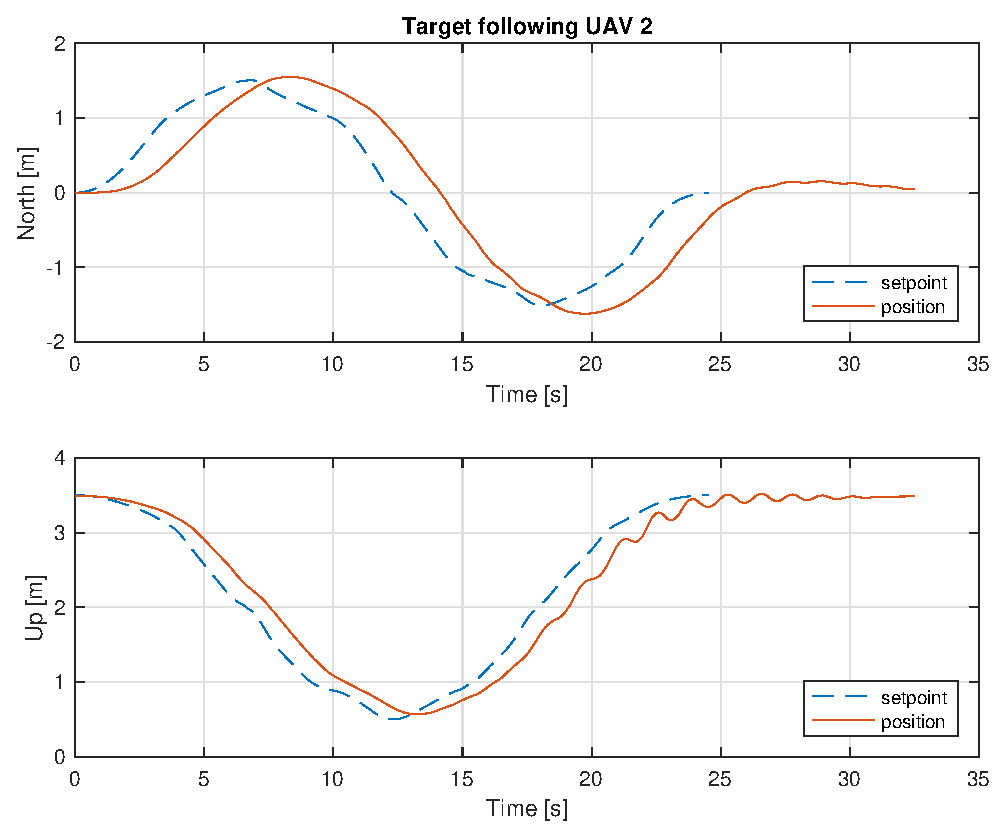
\includegraphics[width=0.7\linewidth]{chapters/chapter-04/figures/following_2.eps}
\caption{Target following drone 2}
\label{fig:following_2}
\end{figure}

There are some delays due to the time needed to the autopilot to follow
the target, but the drones are capable of doing that.
Indeed, they arrive at the same time in their final position.

\begin{figure}
\centering
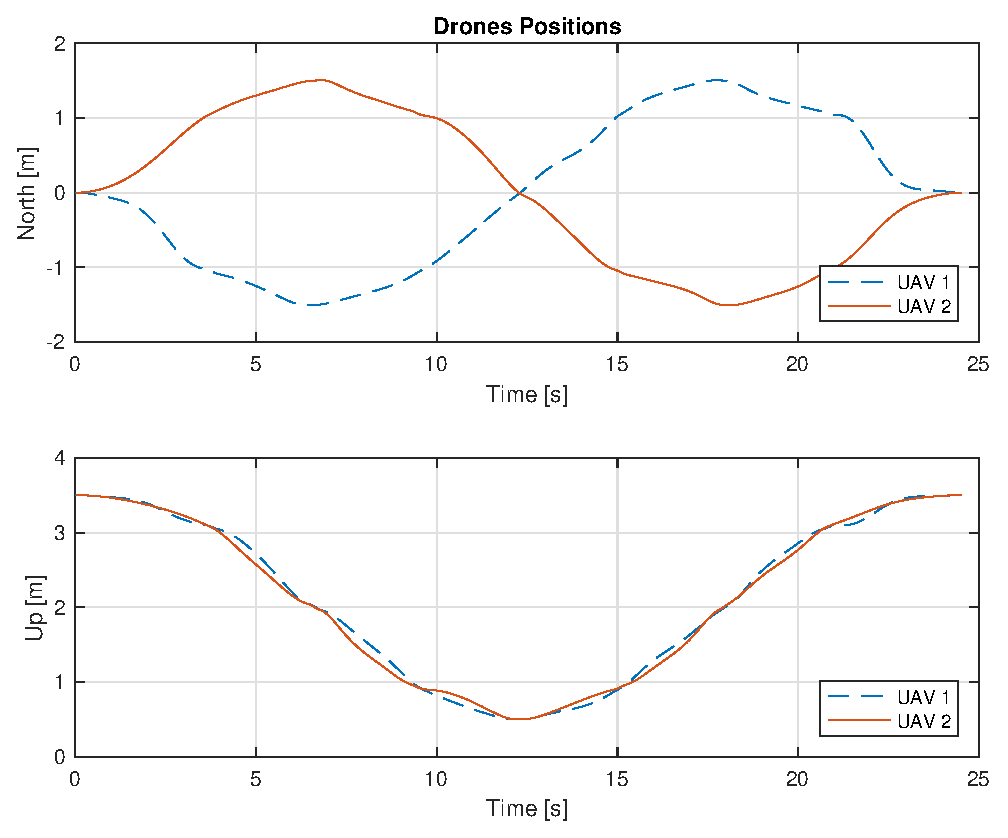
\includegraphics[width=0.7\textwidth]{chapters/chapter-04/figures/overlapped.eps}
\caption{Two drones positions over time}
\label{fig:overlapped}
\end{figure}

If we also consider the figure \ref{fig:overlapped}, we can see that both the drones
are synchronized during the execution of the mission. In the next cases, we will
add disturbances in order to make more evident the effects of the algorithm.


\section{First disturbance}
In this scenario, we use the same trajectory as before (figure \ref{fig:trajectory}),
but in this case we stop one of the two drones and the other will follow it.
We can show the disturbance applied at time 11s to the first drone in the figure \ref{fig:disturbance}.

\begin{figure}
\centering
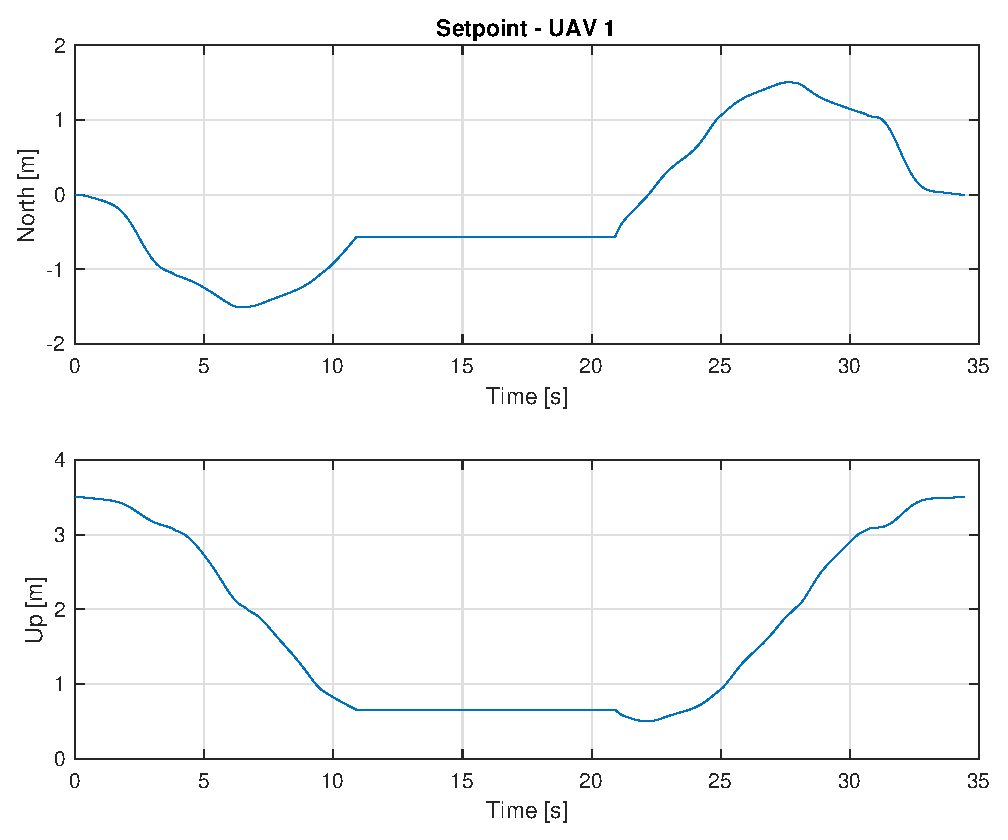
\includegraphics[width=0.7\textwidth]{chapters/chapter-04/figures/pos_1.eps}
\caption{Disturbance}
\label{fig:disturbance}
\end{figure}

We can now see how the two drones execute the mission. The second drone tries to
go on, when the first is interrupted, but then the consensus stops it. The plots are
shown in the figures \ref{fig:following_1_1} and \ref{fig:following_2_1}.

\begin{figure}
\centering
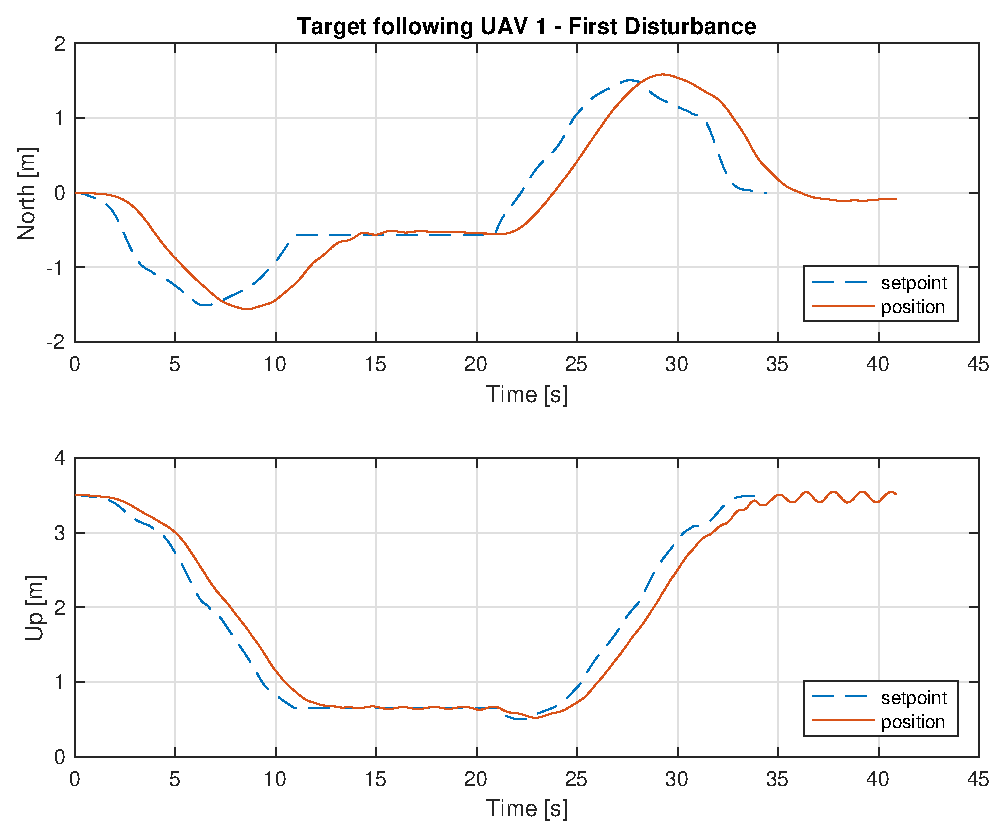
\includegraphics[width=0.7\linewidth]{chapters/chapter-04/figures/following_1_1.eps}
\caption{Target following drone 1}
\label{fig:following_1_1}
\end{figure}

\begin{figure}
\centering
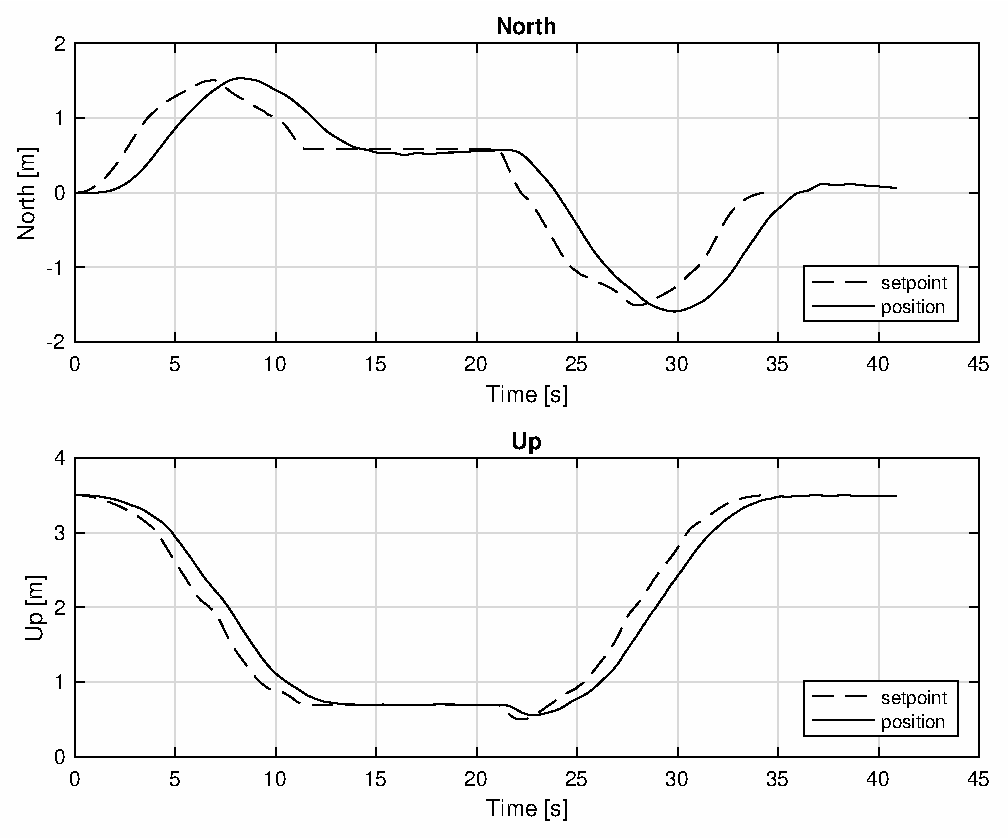
\includegraphics[width=0.7\linewidth]{chapters/chapter-04/figures/following_2_1.eps}
\caption{Target following drone 2}
\label{fig:following_2_1}
\end{figure}

At the end we represent a graph in which we plot the positions of the two drones overlapped
(figure \ref{fig:overlapped_1}).

\begin{figure}
\centering
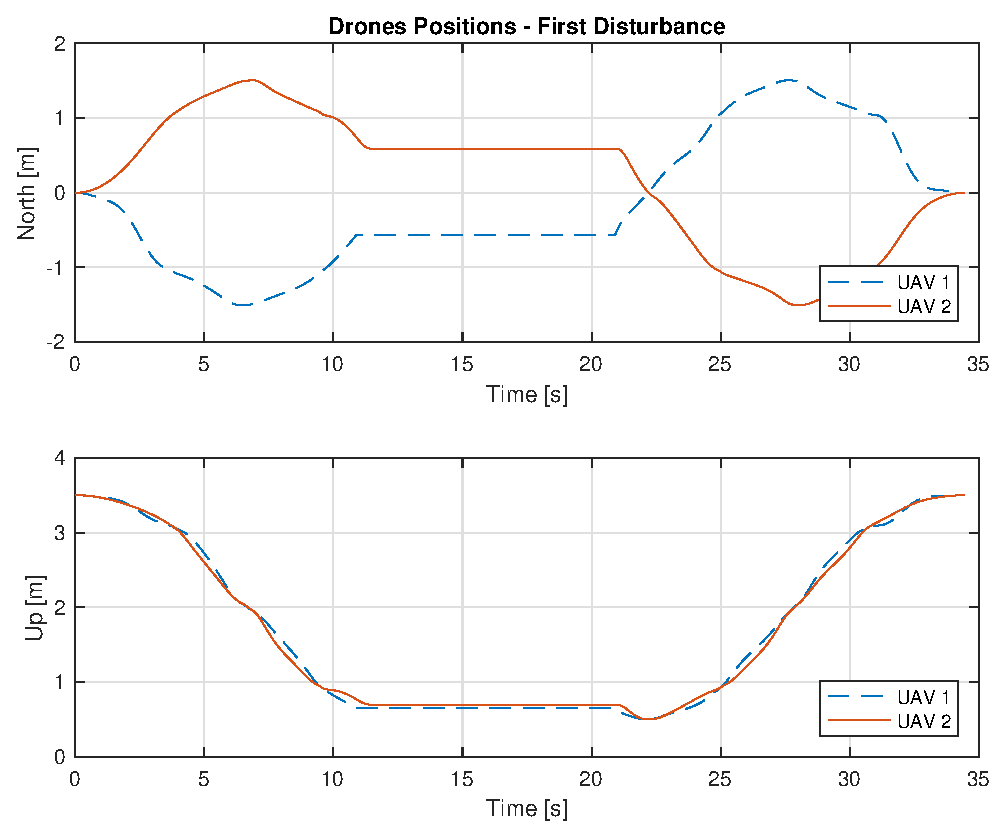
\includegraphics[width=0.7\textwidth]{chapters/chapter-04/figures/overlapped_1.eps}
\caption{Two drones positions over time}
\label{fig:overlapped_1}
\end{figure}


\section{Second disturbance}
The trajectory used is always the same (figure \ref{fig:trajectory}), but this time
the disturbance is different. Now we force one drone to go back through the trajectory
which has travelled so far.
After the disturbance, the drone can resume the trajectory and complete the mission.
We can see the effect of the disturbance on the trajectory in the figure \ref{fig:disturbance_2}.

\begin{figure}
\centering
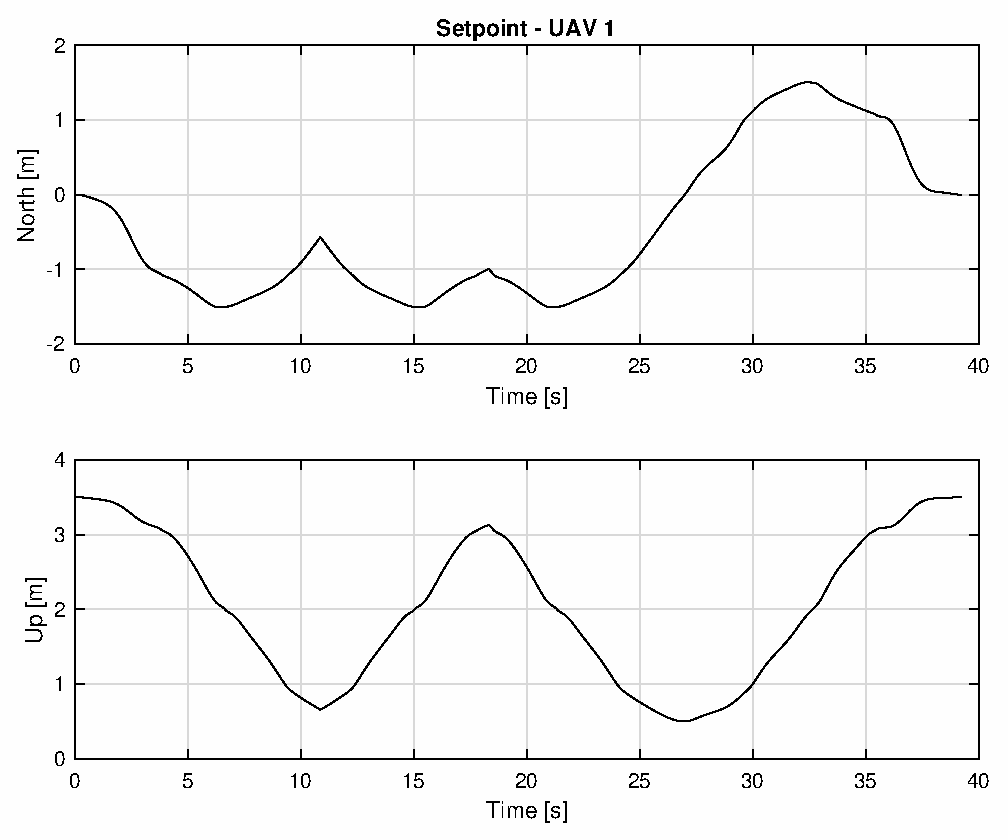
\includegraphics[width=0.7\textwidth]{chapters/chapter-04/figures/pos_2.eps}
\caption{Disturbance}
\label{fig:disturbance_2}
\end{figure}

At time 11s the disturbance starts and the drone start to go back. At time 26s,
the drone is returned to the position where the disturbance is started.

In this situation, the other drone recognizes that the other machine is going back
for an unknown reason and it starts to follow it. We can see how the mission is done
by the two drones in the pictures \ref{fig:following_1_2} and \ref{fig:following_2_2}.

\begin{figure}
\centering
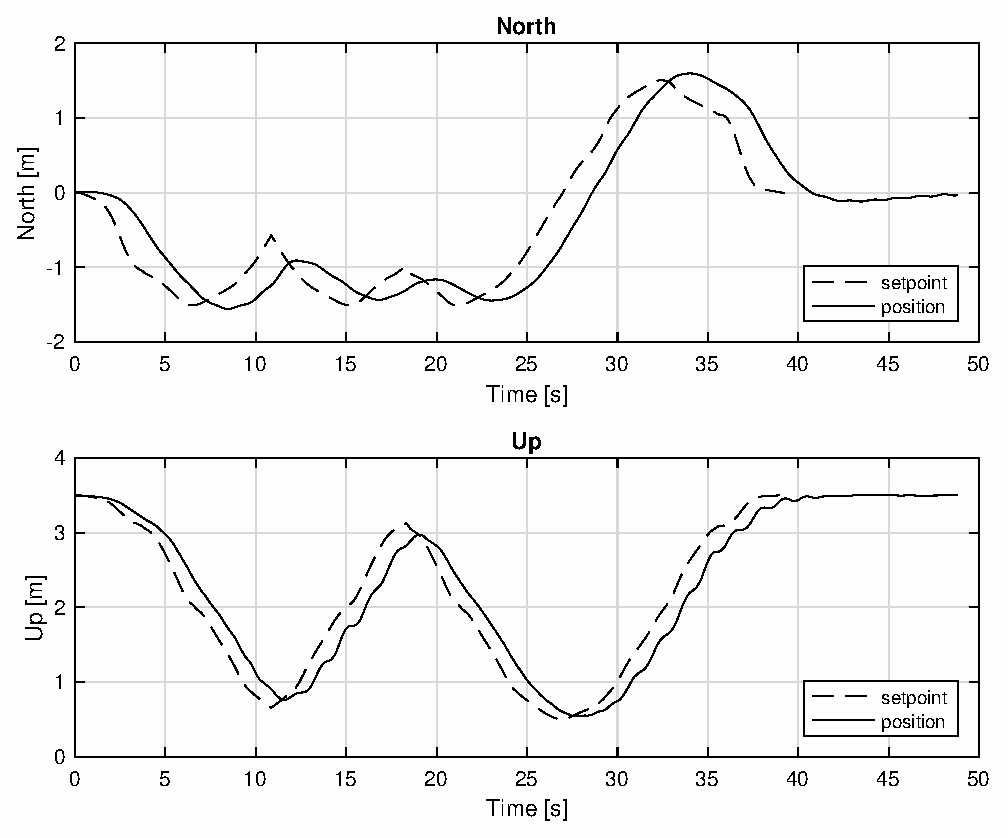
\includegraphics[width=0.7\linewidth]{chapters/chapter-04/figures/following_1_2.eps}
\caption{Target following drone 1}
\label{fig:following_1_2}
\end{figure}

\begin{figure}
\centering
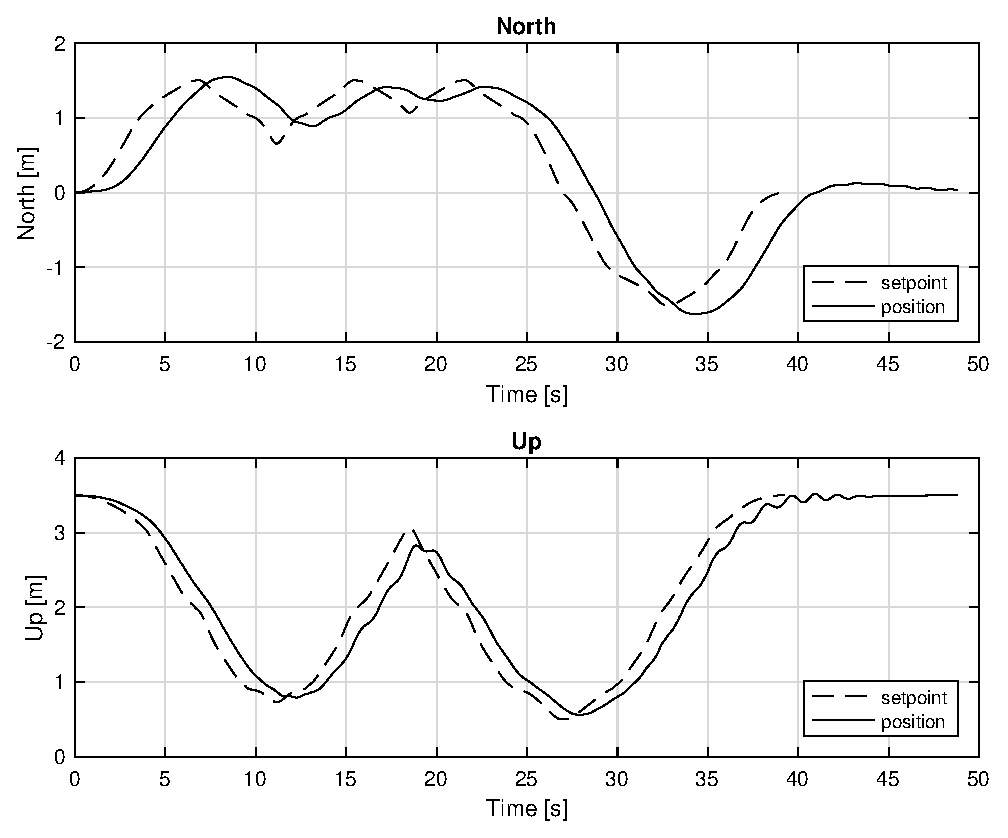
\includegraphics[width=0.7\linewidth]{chapters/chapter-04/figures/following_2_2.eps}
\caption{Target following drone 2}
\label{fig:following_2_2}
\end{figure}

At the end we represent a graph in which we plot the positions of the two drones overlapped
(figure \ref{fig:overlapped_2}).

\begin{figure}
\centering
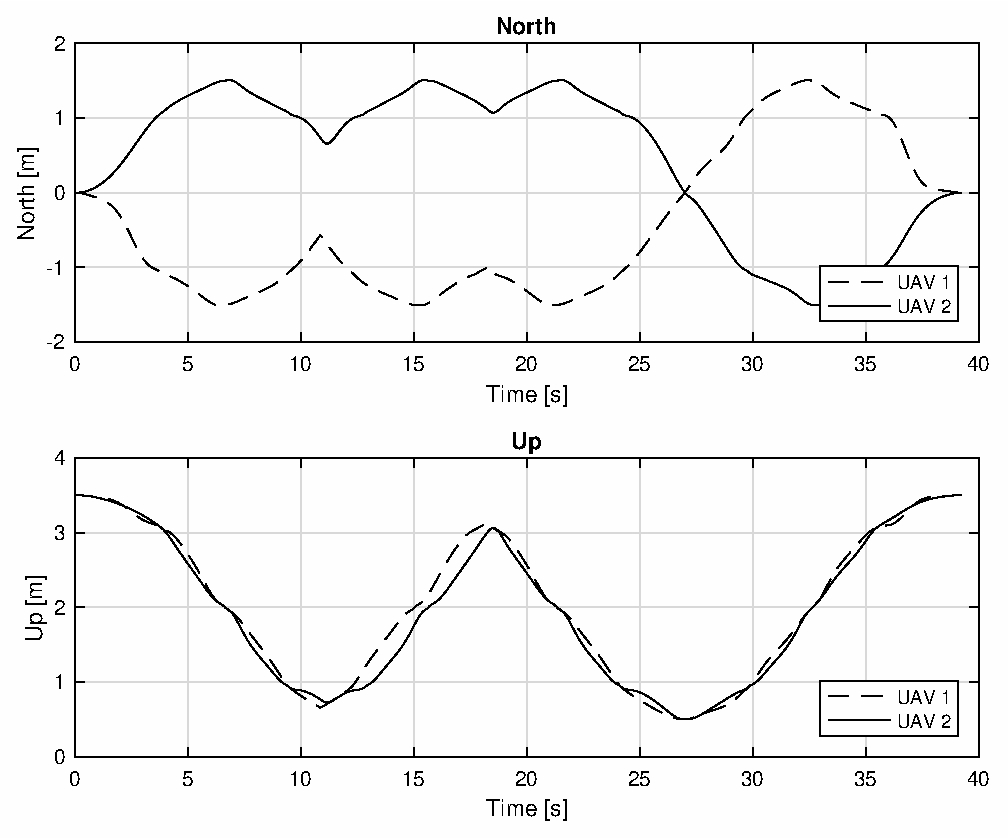
\includegraphics[width=0.7\textwidth]{chapters/chapter-04/figures/overlapped_2.eps}
\caption{Two drones positions over time}
\label{fig:overlapped_2}
\end{figure}
